\subsection{相机参数}
本小节将会结合相机的结构去介绍相机的各种参数。
\subsubsection{感光元件}
相机目前的主流的感光元件有CCD(电荷耦合)和CMOS(互补金属氧化物半导体)两种。

\textbf{CCD}

Charge Coupled Device,它使用一种高感光度的半导体材料制成,由许多感光单位组成,通常以百万像素为单位。当CCD表面受到光线照射时,每个感光单位会将电荷反映在组件上,即把光线转变成电荷,电荷在像素之间依次传递,最终集中到串联寄存器,转换为电压信号,然后放大,经模数转换后形成数字信号。而后数字信号,经过压缩后保存在相机内部的闪速存储器或内置硬盘卡中。有能力生产CCD 的公司分别为:索尼、飞利浦、柯达、松下、富士、夏普,大半是日本厂商。

\textbf{CMOS}

Complementary Metal-Oxide Semiconductor,和CCD一样同为在数码相机中可记录光线变化的半导体。CMOS的制造技术和一般计算机芯片没什么差别,主要是利用硅和锗这两种元素所做成的半导体,使其在CMOS上共存着带N(带–电) 和 P(带+电)级的半导体,这两个互补效应所产生的电流即可被处理芯片纪录和解读成影像。
每个像元都有独立的节点,转换为电压信号,然后放大,经模数转换后形成数字信号。

\textbf{CCD与CMOS的区别}

1.成像过程

CCD仅有一个(或少数几个)输出节点统一读出,其信号输出的一致性非常好。

CMOS中每个像素都有各自的信号放大器,各自进行电荷-电压转换,信号输出的一致性较差。

CCD为了读出整幅图像信号,要求输出放大器的信号带宽较宽。

CMOS中,每个像元中的放大器的带宽要求较低,大大降低了芯片的功耗,但数以百万的放大器的不一致性却带来了更高的固定噪声。

2.集成性

CCD中的电路和器件是集成在半导体单晶材料上,工艺较复杂。其仅能输出模拟电信号,需要后续的地址译码器、模数转换器、图像信号处理器处理,并且还需要提供三组不同电压的电源和同步时钟控制电路,集成度非常低。

CMOS能将图像信号放大器、信号读取电路、A/D转换电路、图像信号处理器及控制器等集成到一块芯片上,集成度高,芯片级相机的概念也由此产生。

3.速度

CCD采用光敏元输出,只能按规定的程序输出,速度较慢。

CMOS有多个电荷-电压转换器和行列开关控制,读出速度较快。此外,CMOS的地址选通开关可随机采样,实现子窗口输出,在仅输出子窗口图像时可获得更高的速度。

4.噪声

CCD采用PN结或二氧化硅隔离层隔离噪声,成像质量相对CMOS有一定的优势。

CMOS的集成度较高,各元件、电路之间距离很近,干扰较为严重,噪声对图片质量影响很大。

5.功耗

CCD需要3路电源来满足特殊时钟的需求,功耗较大。

CMOS只需一个电源供电,功耗仅为CCD的1/10。

\textbf{总结}

目前,市场销售的数码摄像头中以CMOS感光器件的为主。在采用CMOS为感光元器件的产品中,通过采用影像光源自动增益补强技术,自动亮度、白平衡控制技术,色饱和度、对比度、边缘增强以及伽马矫正等先进的影像控制技术,完全可以达到与CCD摄像头相媲美的效果。

受市场情况及市场发展等情况的限制,摄像头采用CCD图像传感器的厂商为数不多,主要原因是采用CCD图像传感器成本高的影响,同时由于CCD耗电量大,工艺复杂,像素提高难度加大。

\subsubsection{相机感光参数}
调整相机对环境的感光程度,主要有以下三个途径,分别是光圈、快门和ISO。

\textbf{光圈}

通过调整镜头光圈的大小,调整进光量,光圈大小有两种写法:大F写法(F2.8)、小f写法(f/2.8),两种写法完全等价,例如F4指的是光圈大小占镜头直径的4分之1。
F后面的数字越大,光圈越小,反之则反。

1.挡位设计

光圈的档位设计是相邻的两档的数值相差1.4倍(2的平方根1.414的近似值)相邻的两档之间。
透光孔直径相差根号2倍,透光孔的面积相差一倍, 底片上形成的影像的亮度相差一倍,维持相同曝光量所需要的时间相差一倍。

所有的光圈挡位有:

f/1.0,f/1.4,f/2.0,f/2.8,f/4.0,f/5.6,f/8.0,f/11,f/16,f/22,f/32,f/44,f/64

2.光圈分类

固定光圈:最简单的相机只有一个园孔的固定光圈

沃特侯瑟光圈:最初的可变光圈只是一系列大小不同的园孔排列在一个有中心轴的圆盘的周围;转动园盘可将适当大小的圆孔移到光轴上,达到控制孔径的效果。十九世记中叶约翰·沃特侯瑟发明这种光圈。

猫眼式光圈:由一片中心有椭圆形或菱形孔的金属薄片平分为二组成,将两片有半椭圆形或半菱形孔的金属薄片对排,相对移动便可形成猫眼式光圈。猫眼式光圈多用于简单照相机。

"虹膜"式光圈:是由多个相互重叠的弧形薄金属叶片组成的,叶片的离合能够改变中心圆形孔径的大小。有些照相机可以借助转动镜头筒上的圆环改变光圈孔径的大小,而有些照相机则是利用微处理器芯片控制微电机自动地改变光圈的孔径。弧形薄金属叶片可多达十八片。弧形薄金属叶片越多,孔径越近圆形。通过电子计算机设计薄金属叶片的形状,可以只用7片薄金属叶,得到近圆形孔径。

瞬时光圈:单反照相机的光圈是瞬时光圈,只在快门开启的瞬间,光圈缩小到预定大小。平时光圈在最大位置。

兼快门光圈:有的简便照相机的光圈兼有快门的功能,这类兼快门光圈大多是双叶片的猫眼式光圈,与单纯猫眼式光圈不同的是:于兼快门光圈平时是完全关闭的:在按下快门的瞬间,双叶片光圈开启到预定的孔径后,保持这孔径到一段预定快门开启时间之后,立刻闭合:如此一来,光圈便又兼快门的功能。

偷懒不放图了先(逃

\textbf{快门}

快门是遮光板,只有当快门打开的时候,底片才能接收到光照。所以快门可以控制进光时间。
快门越块:成像时间越短,被拍摄物品移动的距离越小,图像越清晰。常用于静态拍摄。
反之则反

但是随着相机技术进步,现在相机大部分使用电子快门,常见的电子快门主要有两种,卷帘快门和全局快门

1.卷帘快门

卷帘快门通过逐行扫描的方式从上到下捕获图像,而不是一次性捕获所有像素。这意味着每一行像素的曝光存在微小的时间差。当相机或物体高速移动时,这种逐行扫描可能导致图像失真,形成“果冻效应”
但是其有着成本低,分辨率高的优点,使其在一些需要高分辨率但对动态性能要求不高的应用中非常适用,如静态图像捕捉或家用监控。

卷帘快门导致的果冻效应,其显著程度主要取决于以下几个因素:

*物体的移动速度:移动速度越快,失真越明显。

*物体的大小:大尺寸物体在画面中的扭曲更加明显。

*分辨率:更高的分辨率在相同帧率下行时间更短,相对可以减少失真。

2.全局快门

全局快门(Global Shutter)是一种图像传感器技术,其核心在于能够同时捕获画面中所有像素的信息。与逐行扫描的滚动快门不同,全局快门的所有像素在同一时间曝光,然后一起读取数据,这种同步曝光方式使其在高速运动场景中能够有效消除图像失真现象,如“果冻效应”(rolling shutter effect)。可以将其比作拍照时快门在一瞬间“拍下”整个画面,而非逐行扫描捕捉,确保每一部分都与真实场景一致。

\begin{figure}[H]
    \centering
    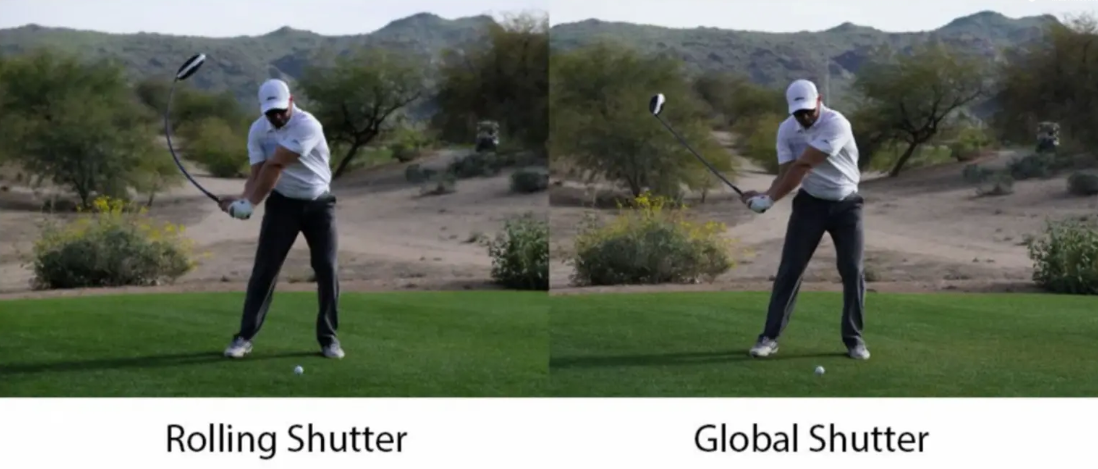
\includegraphics[width=0.7\textwidth]{rolling_shutter.png}
    \caption{快门对比} % 图片标题
    \label{fig:果冻} % 图片标签,用于引用
\end{figure}

总结

静态场景可以使用卷帘快门相机,相同价格下,可以获得更高分辨率的相机,动态场景下,则需要根据情况权衡,优先全局快门相机,其次高帧率,高分辨率的
卷帘快门,在要求不高的程度上,也可以,请根据成本酌情考虑。在笔者眼里,全局快门的缺点就是贵(哭

\textbf{ISO}

感光度,又称为ISO值,是衡量底片对于光的灵敏程度。
对光越灵敏,越适合捕捉暗光线:亮处用小ISO即可,暗处用大ISO。对光越灵敏,意味着所需的进光时间越短:
意味着所需快门的时间越短。所以ISO值上限决定了快门的上限,只有ISO足够大,快门才可以足够快。
意味着曝光量越少。所以ISO越大,图像越模糊,使用较高敏感度通常会导致影像质量降低(较粗的底片颗粒或是较高的影像噪声)。
ISO每差一倍,曝光量差一档,也就是说相差一档光圈或者一档快门。

提高ISO会降低图像质量,所以优先采取其他方法提高亮度。

\subsubsection{图片噪点}
噪点在图像上常表现为一引起较强视觉效果的孤立像素点或像素块。比如上午所提的提高ISO或者相机长时间工作过热等,都可能会导致出现噪点。

图像常见噪声基本上有以下四种,高斯噪声,泊松噪声,乘性噪声,椒盐噪声。

\begin{figure}[H]
    \centering
    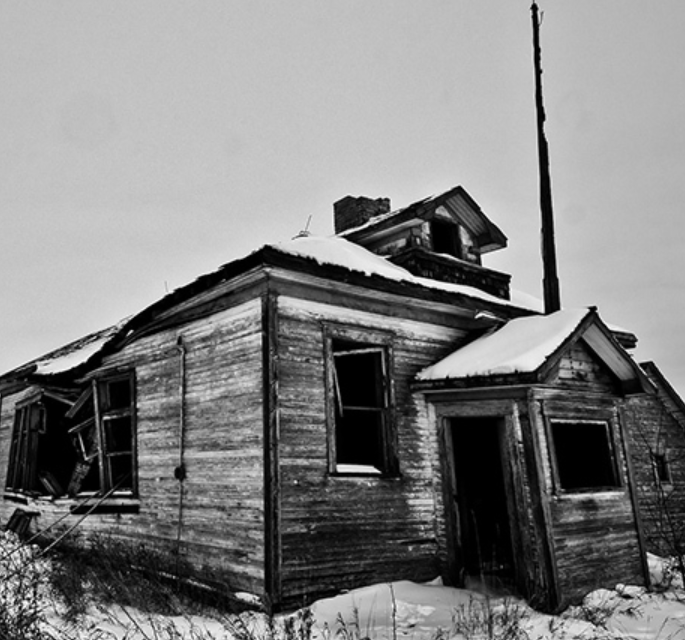
\includegraphics[width=0.6\textwidth]{raw.png}
    \caption{原图} % 图片标题
    \label{fig:原图} % 图片标签,用于引用
\end{figure}

\textbf{高斯噪声}

高斯噪声是指它的概率密度函数服从高斯分布(即正态分布)的一类噪声。如果一个噪声,它的幅度分布服从高斯分布,而它的功率谱密度又是均匀分布的,则称它为高斯白噪声。高斯白噪声的二阶矩不相关,一阶矩为常数,是指先后信号在时间上的相关性。

产生原因:

1)图像传感器在拍摄时市场不够明亮、亮度不够均匀。

2)电路各元器件自身噪声和相互影响。

3)图像传感器长期工作,温度过高。

\begin{figure}[H]
    \centering
    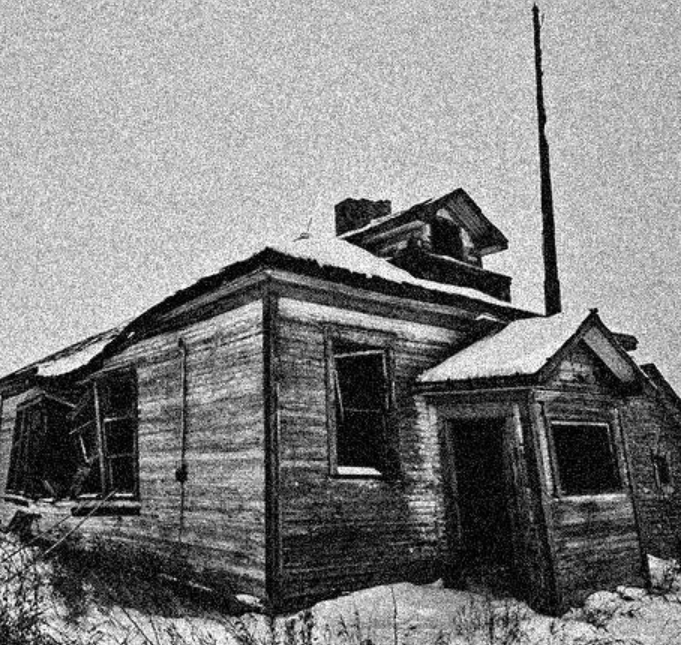
\includegraphics[width=0.6\textwidth]{gaussian.png}
    \caption{高斯噪声} % 图片标题
    \label{fig:高斯噪声} % 图片标签,用于引用
\end{figure}

\textbf{泊松噪声}

泊松噪声,就是符合泊松分布的噪声模型,泊松分布适合于描述单位时间内随机事件发生的次数的概率分布。如某一服务设施在一定时间内受到的服务请求的次数,电话交换机接到呼叫的次数、汽车站台的候客人数、机器出现的故障数、自然灾害发生的次数、DNA序列的变异数、放射性原子核的衰变数等。

\begin{figure}[H]
    \centering
    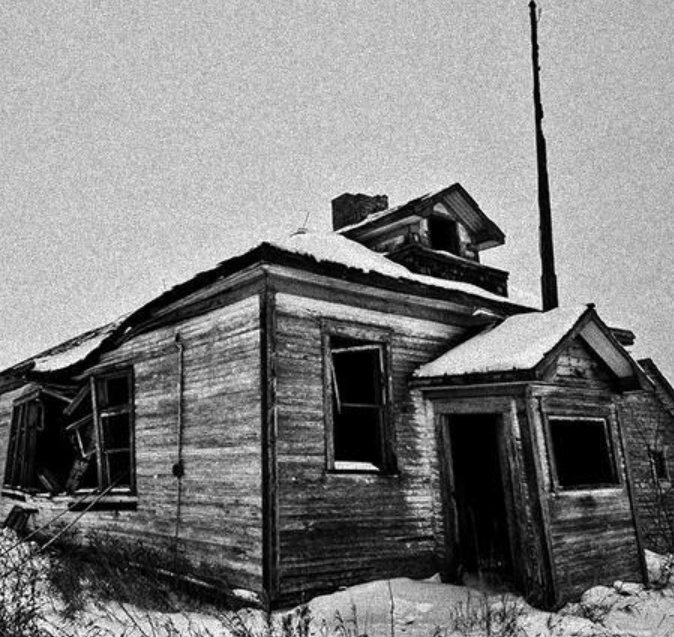
\includegraphics[width=0.6\textwidth]{poisson.png}
    \caption{泊松噪声} % 图片标题
    \label{fig:泊松噪声} % 图片标签,用于引用
\end{figure}

\textbf{乘性噪声}

乘性噪声一般由信道不理想引起,它们与信号的关系是正相关,信号在它在,信号不在他也就不在。

\begin{figure}[H]
    \centering
    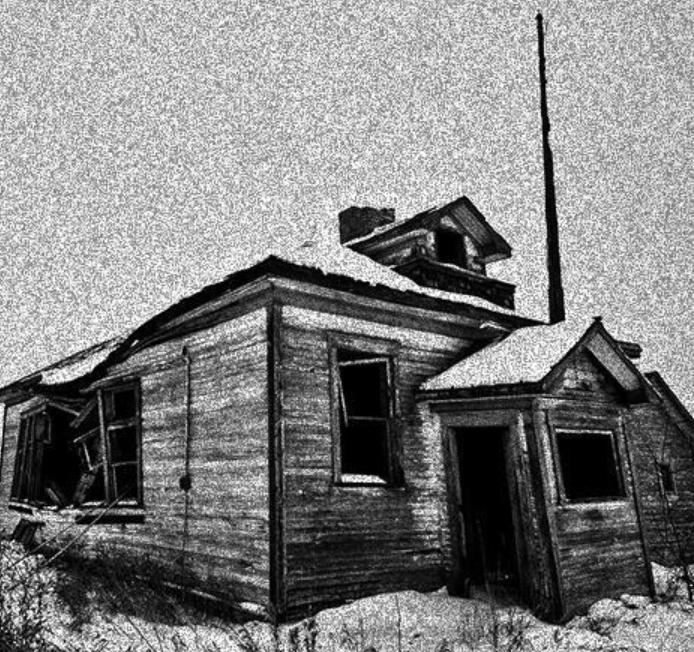
\includegraphics[width=0.6\textwidth]{x.png}
    \caption{乘性噪声} % 图片标题
    \label{fig:乘性噪声} % 图片标签,用于引用
\end{figure}

\textbf{椒盐噪声}

椒盐噪声,椒盐噪声又称脉冲噪声,它随机改变一些像素值,是由图像传感器,传输信道,解码处理等产生的黑白相间的亮暗点噪声。

\begin{figure}[H]
    \centering
    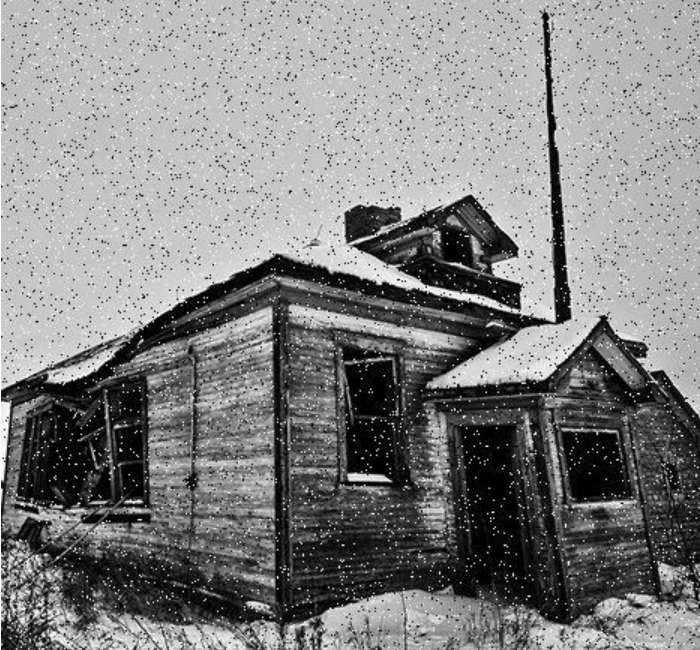
\includegraphics[width=0.6\textwidth]{salt.png}
    \caption{椒盐噪声} % 图片标题
    \label{fig:椒盐噪声} % 图片标签,用于引用
\end{figure}

\subsubsection{相机图片储存格式}
\textbf{1.Bayer格式}

bayer格式图片是伊士曼·柯达公司科学家Bryce Bayer发明的,Bryce Bayer所发明的拜耳阵列被广泛运用数字图像处理。

bayer 格式图片在一块滤镜上设置的不同的颜色,通过分析人眼对颜色的感知发现,人眼对绿色比较敏感,所以一般bayer格式的图片绿色格式的像素是是r和g像素的和。

另外,Bayer格式是相机内部的原始图片, 一般后缀名为.raw。很多软件都可以查看, 比如PS。我们相机拍照下来存储在存储卡上的.jpeg或其它格式的图片, 都是从.raw格式转化过来的。如下图,为bayer色彩滤波阵列,由一半的G,1/4的R,1/4的B组成。

Bayer格式的图片是单通道的。

\textbf{2.RGB格式}

RGB格式是一种多通道图像格式,它将图像分为三个通道,分别为红色通道、绿色通道、蓝色通道。

RGB格式的特点是:

1.每个像素点由三个相邻像素点组成,分别对应三个通道。


RGB格式的优点是:

1.RGB格式的图像可以同时处理红色、绿色、蓝色通道,可以提高图像处理速度。

2.RGB格式的图像占用空间小,占用内存小。

RGB格式的缺点是:

对场景的光照和颜色变化比较敏感,不适用一些需要保持颜色稳定性的应用场景。

\subsubsection{相机伽马值}

所谓伽玛校正就是对图像的伽玛曲线进行编辑,以对图像进行非线性色调编辑的方法,检出图像信号中的深色部分和浅色部分,并使两者比例增大,从而提高图像对比度效果。计算机绘图领域惯以此屏幕输出电压与对应亮度的转换关系曲线,称为伽玛曲线(Gamma Curve)。

在不使用伽马校正去产生JPG图像意味着亮度等级水平在进行8位的转换时会有一定的损失,就会产生“台阶”效果。通过调校亮度的分布就是进行伽马校正意味着那些效果会得到补偿修复。gamma校正的意义就在于将人眼感受到的灰度值, 转换到自然界真正的灰度值(因为人不是测量器, 人只能感受和比较)

\textbf{gamma校正原理}

假设图像中有一个像素,值是 200 ,那么对这个像素进行校正必须执行如下步骤: 
  1. 归一化 :将像素值转换为 0 ~ 1 之间的实数。算法如下:( i + 0. 5)/256 这里包含 1 个除法和 1 个加法操作。对于像素 A 而言,其对应的归一化值为0. 783203 。 

  2. 预补偿 :根据公式, 求出像素归一化后的 数据以1/gamma为指数的对应值。这一步包含一个求指数运算。若gamma值为2. 2 ,则1 /gamma为0. 454545 , 对归一化后的A值进行预补偿的结果就是0. 783203 \^ \ \ \   0. 454545 = 0. 894872。 

  3. 反归一化 :将经过预补偿的实数值反变换为0~255之间的整数值。具体算法为 : f*256 - 0. 5  此步骤包含一个乘法和一个减法运算。续前例, 将A的预补偿结果0. 894872代入上式, 得到A预补偿后对应的像素值为  228 , 这个  228  就是最后送 入显示器的数据。

  
  如上所述如果直接按公式编程的话,假设图像的分辨率为 800*600 ,对它进行 gamma 校正,需要执行 48 万个浮点数乘法、除法和指数运算。效率太低,根本达不到实时的效果。 
  针对上述情况,提出了一种快速算法,如果能够确知图像的像素取值范围,例如, 0 ~ 255 之间的整数  , 则图像中任何一个像素值只能 是  0  到  255  这  256  个整数中的某一个 ; 在  gamma 值 已知的情况下  ,0 ~ 255  之间的任一整数  , 经过“归一 化、预补偿、反归一化”操作后 , 所对应的结果是唯一的  , 并且也落在  0 ~ 255  这个范围内。
  如前例, 已知gamma值为2. 2,像素A的原始值是200,就可求得经gamma校正后A对应的预补偿值为  228 。基于上述原理  , 我们只需为  0 ~ 255  之间的每个整数执行一次预补偿操作  , 将其对应的预补偿值存入一个预先建立的  gamma  校正查找表 (LUT:Look Up Table) , 就可以使用该表对任何像素值在  0 ~ 255  之 间的图像进行  gamma  校正。
 
\begin{figure}[H]
    \centering
    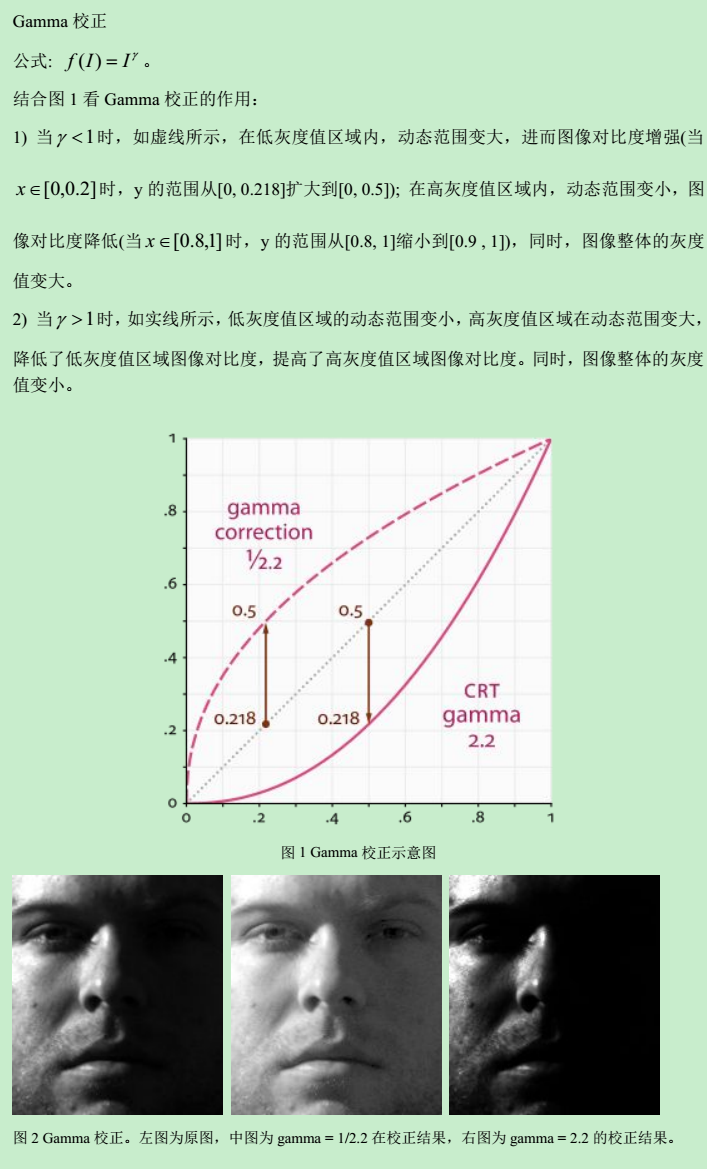
\includegraphics[width=0.95\textwidth]{gamma.png}
    \caption{伽马矫正} % 图片标题
    \label{fig:伽马矫正} % 图片标签,用于引用
\end{figure}

\subsubsection{相机景深}
景深(depth of field)定义:摄影机镜头或其他成像器前沿能够取得清晰图像的成像所测定的被摄物体前后距离范围。通俗讲即被拍摄物体对焦点(focus point)平面处的景物,在胶片上会形成清晰影像,在对焦点平面的前方某处到其后方某处有一个范围,其内的景物都能形成清晰影像,这一范围称为景深,讨论景深,一般我们用“深浅”形容,即浅景深(narrow depth of field)或大景深(large depth of field)。

\textbf{景深的原理}

理解景深原理前,我们必须明白一件事:当我们对焦时,其实只有一个平面是真正合焦的。这个平面与像平面(可以简单理解为胶片或者传感器平面)平行。凡是在这个平面之前或者之后的都不是合焦状态。合焦平面上物体某点发出不同角度的光在像平面成像都汇聚于一点,而非合焦物体的某点发出不同角度的光会落在像平面不同点上,形成一个模糊圆,这个圆术语叫做弥散圆(circle of confusion)。

\begin{figure}[H]
    \centering
    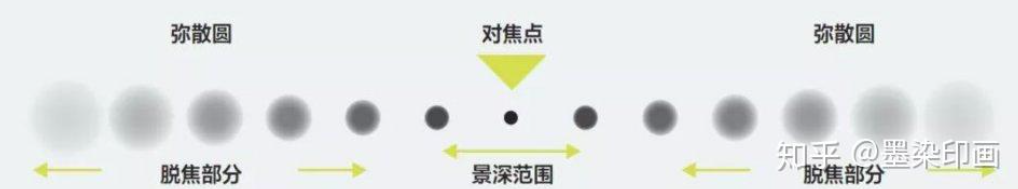
\includegraphics[width=0.95\textwidth]{diffuse_circle.png}
    \caption{弥散圆} % 图片标题
    \label{fig:弥散圆} % 图片标签,用于引用
\end{figure}
如果弥散圆小到人眼无法鉴别(或者说弥散圆直径小于传感器像元的大小),模糊圆可被视为点的成像,看起来就和对上焦的东西一样清晰,此无法分辨的弥散圆称为容许弥散圆(permission circle of confusion)。在被摄物体(对焦点或合焦平面)前后纵深,有一段距离,其影像在像平面的模糊程度肉眼无法分辨,比较清晰,都在容许弥散圆限定范围内,它们之间距离称为景深。

\textbf{*景深的计算}

\begin{figure}[H]
    \centering
    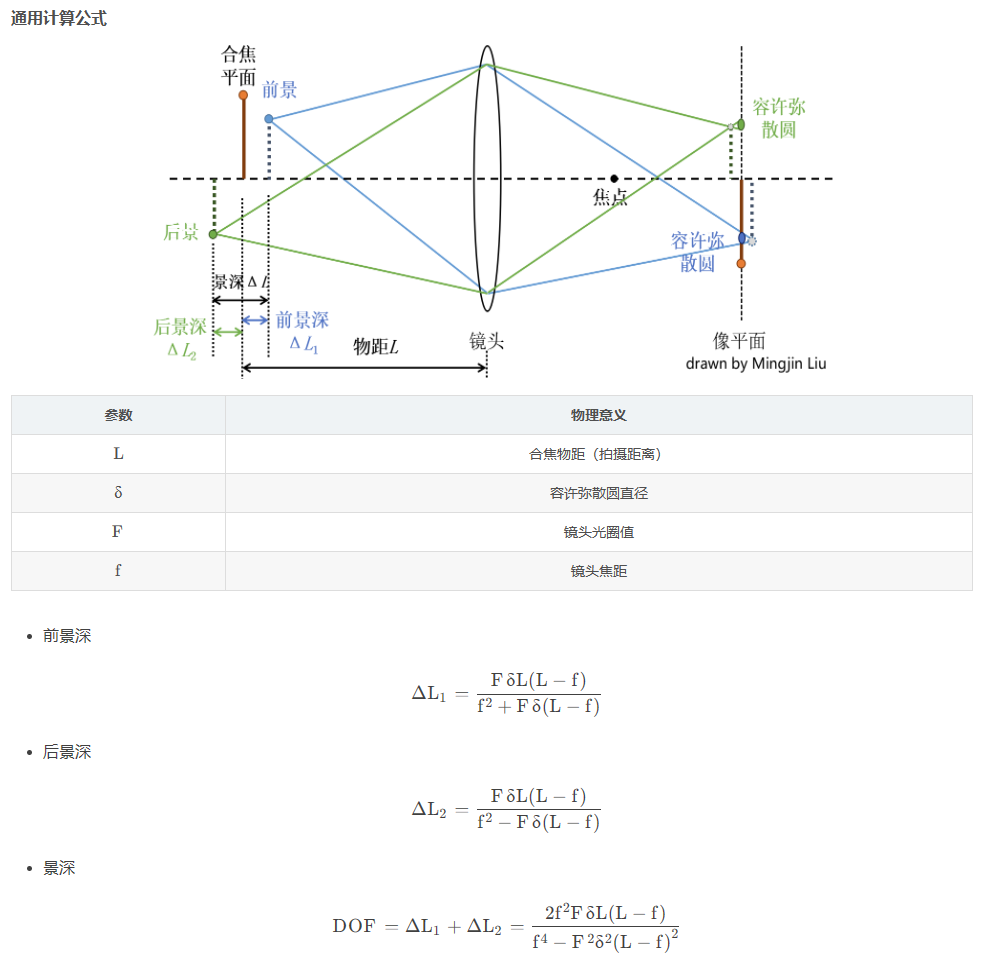
\includegraphics[width=1\textwidth]{depth_of_field.png}
    \caption{景深计算} % 图片标题
    \label{fig:景深计算} % 图片标签,用于引用
\end{figure}
可见,前景深,小于后景深。
\begin{figure}[H]
    \centering
    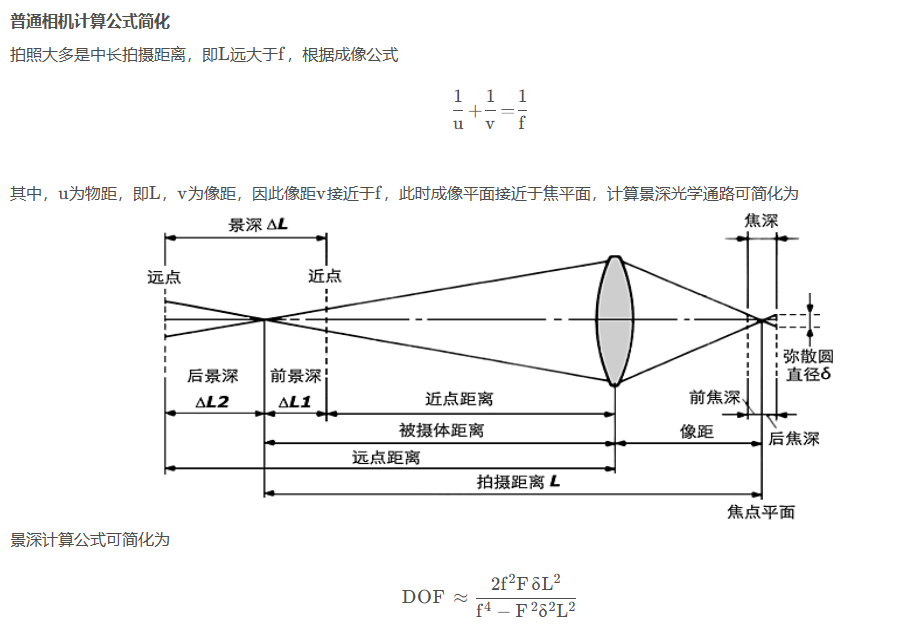
\includegraphics[width=0.95\textwidth]{simple.png}
    \caption{景深简化计算} % 图片标题
    \label{fig:景深简化计算} % 图片标签,用于引用
\end{figure}
\textbf{景深的影响因素}

镜头光圈:光圈越大,景深越小;光圈越小,景深越大;

镜头焦距:镜头焦距越长,景深越小;焦距越短,景深越大;

拍摄距离:距离越远,景深越大;距离越近,景深越小。
\begin{figure}[H]
    \centering
    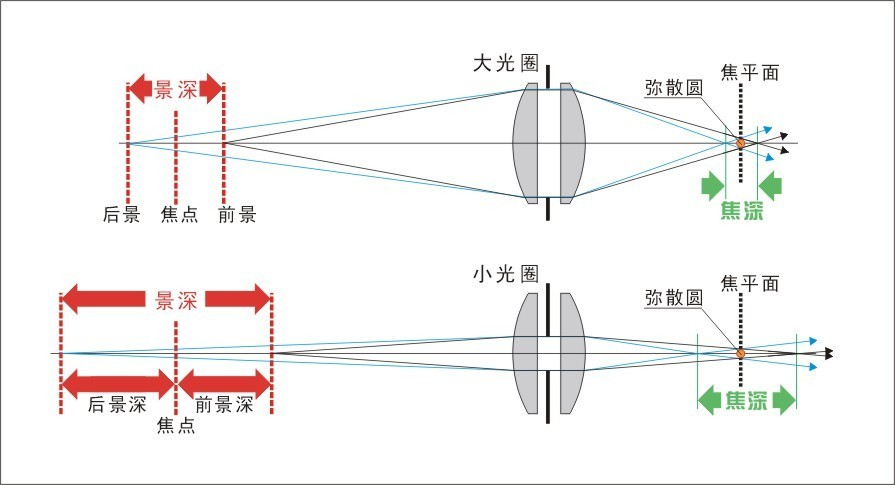
\includegraphics[width=0.75\textwidth]{aperture.png}
    \caption{光圈} % 图片标题
    \label{fig:光圈} % 图片标签,用于引用
\end{figure}
\subsubsection{焦段的选择}



相机镜头的选择

镜头参数

光圈大小之类的

\subsection{相机畸变模型}
\subsubsection{针孔相机}
\subsubsection{鱼眼相机}
\subsubsection{广角相机}

相机标定介绍
几种常用的标定板/棋盘,圆点,aruco,charuco

ros包标定 opencv标定 手写标定
每种给出文档,手写标定研究一下,写出来给

单目标定,双目标定,动态标定,在线标定,自标定(这两个有区别),无标定板标定等多种类型的标定

\subsubsection{相机选购}
几种常见的相机像素单位,商家说高清,不一定真高清

相机帧率不一定是当前的分辨率,可能指的是120hz的时候480p,1080p的时候其实只有30hz

分清黑白,分辨率等参数

定焦,自动调焦AF/FF

\subsection{HDR实现}
\subsection{多相机同步}
